In today's large-scale HPC systems, an increasing portion of the computing capacity is wasted due to failures and recoveries. It is expected
that future exascale machines,  featuring a computing capability of exaFLOPS, will decrease the mean time between
failures to a few hours, making fault tolerance extremely challenging. 
Enabling Shadow Replication for resiliency in extreme-scale computing 
brings about a number of challenges and design decisions, including the applicability of this concept to a large number of 
tasks executing in parallel, the effective way to control shadows' execution rates, and the runtime mechanisms and 
communications support to ensure efficient coordination between a 
main and its shadow.


Taking into consideration the main characteristics of compute-intensive and highly-scalable applications, we design a novel fault tolerance model of \textit{Leaping Shadows}. Leaping Shadows is a Shadow Replication based model that associates a suite of shadows
to each main process. To achieve fault tolerance, shadows
execute simultaneously with the mains, but on different
nodes. Furthermore, to save power, shadows execute at a
lower rate than their associated mains. When a main fails,
the corresponding shadow increases its execution rate to speed up recovery.
This chapter focuses on tolerating crash failures under the fail-stop fault model, 
whereby a failed process halts and its internal state and
memory content are irretrievably lost. As a consequence, each main process is replicated with one shadow.  A study of tolerating silent failures will be discussed in Chapter~\ref{chapter:sdc}. 

To achieve higher efficiency and better scalability, however, we adopt radically different methodologies in the design of Leaping Shadows from the Shadow Replication model.
In the original Shadow Replication, shadows are designed to
substitute for their associated mains when failure occurs. The tight coupling and ensuing fate sharing between a main and its shadow increase the implementation complexity and reduce the efficiency of
the system to deal with failures.
In this new model, we deviate from the original design, and use each shadow as a ``rescuer", whose role is to restore the associated main
to its exact state before failure.

Instead of using DVFS to achieve the desired execution rates, this work applies collocation to shadowing for the first time, in order to simultaneously save power and computing resources. In addition, two issues, \textit{divergence} and \textit{vulnerability}, have been identified that limit Shadow Replication's effectiveness in large-scale, failure-prone computing environments. This chapter discusses innovative techniques of {\it leaping} and {\it  rejuvenation} as the provided solutions, respectively. %, to achieve higher efficiency and better scalability.

\section{Shadow Collocation}
\label{sec:shadow_collocation}
In HPC, throughput consideration requires that the rate of the main, $\sigma_m$, and the rate of the shadow after failure, 
$\sigma_s^a$, be set to the maximum. 
The initial execution rate of the shadow, $\sigma_s^b$, however, can be derived by balancing the trade-offs between delay and energy.
For a delay-tolerant, energy-stringent application, $\sigma_s^b$ is set to 0, and the shadow starts executing only upon failure of the main process. 
For a delay-stringent, energy-tolerant application, the shadow starts executing at $\sigma_s^b=\sigma_m$ to guarantee the completion of the task at the specified time $t_m$, regardless of when the failure occurs.  
In addition, a broad spectrum of delay and energy trade-offs in between can be explored either empirically or by using optimization frameworks for delay and energy tolerant applications.


To control the shadows' execution rates, DVFS can be applied while each shadow resides on one processor exclusively. 
The effectiveness of DVFS, however, may be markedly 
limited by the granularity of voltage control, the number of frequencies available, and the negative effects on 
reliability~\cite{Eyerman:2011:FDU:1952998.1952999,Keller:EECS-2015-257,chandra2008defect,zhao2008reliability}. 
An alternative is to collocate shadows.
We use the term processor to represent the resource allocation unit (e.g., a CPU core, a multi-core CPU, or a cluster node), so that our discussion is agnostic to the granularity of the hardware platform. While each main process occupies a processor,  we collocate multiple shadows on each processor and use time sharing to achieve the desired execution rates.
%Compared to DVFS, this approach simultaneously reduces the number of processors required and the corresponding power consumption. 


To execute an application of $M$ parallel tasks, $N=M+S$ processors are required, where $M$ is a multiple of $S$. Each main is allocated one processor (referred to as \textit{main processor}), while $\alpha=M/S$ (referred to as \textit{collocation ratio}) shadows are collocated on a processor (referred to as \textit{shadow processor}). 
The $N$ processors are grouped into $S$ sets, each of which we call a \textit{shadowed set}. Each shadowed set contains $\alpha$ main processors and 1 shadow processor.
This has been illustrated in Figure~\ref{fig:sc_mapping}.  

Contrary to traditional process replication, shadow collocation reduces
the number of processors required to achieve fault-tolerance,
thereby reducing power and energy consumption. Furthermore, the collocation ratio can be adapted to reflect the
propensity of the system to failure. This flexibility, however,
comes at the increased cost of memory requirement at the
shared processor. It is to be noted that this limitation is not
intrinsic to Leaping Shadows, as in-memory checkpoint/restart and multilevel checkpoint/restart also require additional memory to store checkpoints.

Under Shadow Replication, collocation has an important ramification with respect to the resilience of the system. Specifically, only
one failure can be tolerated in each shadowed set. If a shadow processor fails, all the shadows in the 
shadowed set will be lost, although this does not interrupt the execution of the mains. 
On the other hand, if a main processor fails, the associated shadow will be promoted to a new main, and all 
the other collocated shadows will be terminated to speed up the new main.
Consequently, a failure, either in main or shadow processor, will result in losing all the shadows in the shadowed set, thereby losing the tolerance to any other failures. After the first failure, a shadowed set becomes \emph{vulnerable}. To address this issue, Leaping Shadows applies rejuvenation, to be discussed in Section~\ref{sec:rejuvenation}, to maintain a persistent level of system resilience.



\section{Leaping}
\label{sec:leaping_shadows}

In the basic form of Shadow Replication, failures can
have a significant impact on the performance. Since a
shadow executes at a lower rate than its associated main,
a computational \textit{divergence} will occur between the pair of processes. As shown in Figure~\ref{fig:divergence}, the larger this divergence, the more time the lagging shadow will need to ``catch up" in the case of a failure, introducing delay to the recovery process. 
This problem deteriorates as dependencies incurred by messages and synchronization barriers would propagate the delay of one task to others. 
At the same time, divergence has another side-effect in message passing systems. Specifically, forwarding messages from mains to shadows in a message passing system will cause undesired message accumulation. Similarly, the message buffer will bear higher pressure as divergence increases. 

\begin{figure}[!t]
	\begin{center}
			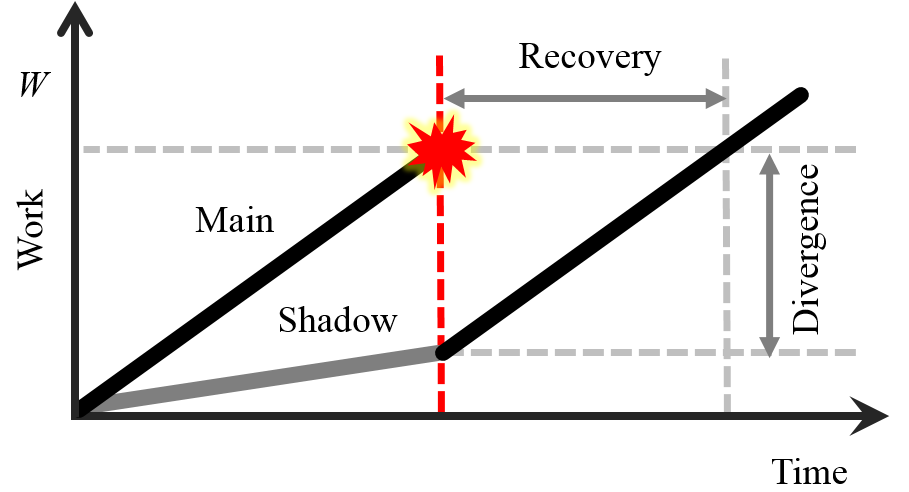
\includegraphics[width=\columnwidth]{Figures/divergence}
	\end{center}
	\caption{Illustration of divergence between a main and its shadow.}
	\label{fig:divergence}
\end{figure}
 
Fortunately, the association with the mains provides an unique opportunity for the shadows to benefit from the faster execution of their mains. By copying the state of a main to its shadow, which is similar to the process of storing a checkpoint in a buddy in \cite{zheng_2004_ftccharm}, forward progress is achieved for the shadow with minimized time and energy. This technique, referred to as \textit{leaping}, effectively limits the divergence between main and shadow. 
As a result, there is no need of concern for buffer overflow, and the recovery time after a failure, which depends on the divergence between the failing main 
and its shadow, is also reduced. 


While recovery may lead to delay due to divergence, we opportunistically overlap shadow leaping with failure recovery to avoid extra overhead. 
Assuming a failure occurrence at time $t_f$, Figure~\ref{fig:leap} shows the concept of leaping overlapped with failure recovery. 
Upon failure of a main process, its associated shadow speeds up to minimize the impact of failure recovery on the other tasks' progress, as illustrated in Figure~\ref{fig:jump1}. 
At the same time, as shown in Figure~\ref{fig:jump2}, the remaining main processes are blocked
at the next synchronization point, which is assumed to take
place shortly after $t_f$. 
Leaping opportunistically takes advantage of this idle time to {\it leap forward} the shadows, so that  
all processes, including shadows, can resume execution from a consistent point afterwards. 
Leaping increases the shadow's rate of progress, at a minimal energy cost. Consequently, it reduces significantly the likelihood of a shadow falling excessively behind, thereby ensuring fast recovery while minimizing the total energy consumption. Note that leaping is applicable, whether shadows are collocated or use DVFS. However, in the case of collocation, the leaping for some shadows could not overlap with the recovery. This will be further discussed in the next section when we integrate leaping with rejuvenation.  

\begin{figure}[!h]
	\begin{center}
        \subfigure[Faulty task behavior.]
		{
			\label{fig:jump1}
			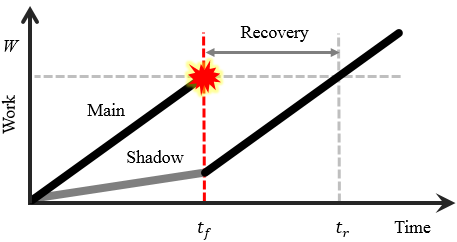
\includegraphics[width=0.6\columnwidth]{Figures/exe_leap_1}
		}
		\subfigure[Non-faulty task behavior.]
		{
			\label{fig:jump2}
			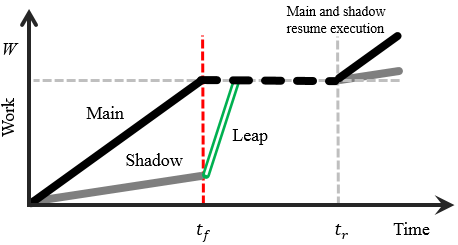
\includegraphics[width=0.6\columnwidth]{Figures/exe_leap_2}
		}
	\end{center}
	\caption{Illustration of shadow leaping after a failure.}
	\label{fig:leap}
\end{figure}

The main objective of leaping is to ensure forward
progress in the presence of failure. However, later on we have identified that leaping is useful in a variety of scenarios. Correspondingly, we define multiple types of leaping, each of which applies to a particular scenario. Above mentioned leaping is referred to as \textit{failure-induced leaping}, as it is triggered by a failure. As also mentioned above, message buffer pressure increases with divergence in message passing systems. If failure-induced leaping is not frequent enough, there may be a need to force a leaping to avoid buffer overflow, thus this type of leaping is referred to as \textit{buffer-forced leaping}. Furthermore, in following chapters we will demonstrate that leaping can be used to achieve forward progress, for both shadow and main processes, in another two scenarios, resulting in \textit{rejuvenation-induced leaping} and \textit{voting-induced leaping}. In all scenarios, leaping always takes
place between a main and its associated shadow, and thus
does not require global coordination. The process which
provides the leaping state is referred to as the \textit{leap-provider},
while the process which receives the leaping
state and rolls forward is referred to as the \textit{leap-recipient}.



\section{Rejuvenation}
\label{sec:rejuvenation}
Another shortcoming of Shadow Replication is that failures can impact the resilience of the system. 
Upon failure of a main, the system can only rely on an
``orphan" shadow to complete the task. 
This is even worse when shadows are collocated. As discussed in Section~\ref{sec:shadow_collocation}, each shadowed set can only tolerate a single failure. 
A trivial approach to
address this shortcoming is to associate a ``suite" of shadows
with each main. Such an approach, however, is resource
wasteful and costly in terms of energy consumption. Instead, Leaping Shadows embraces rejuvenation techniques to improve resource efficiency, when a processor on which a failure occurred can be rebooted to start new processes\footnote{Equivalently, a spare processor can be used for this purpose.}. %This assumption also holds for checkpointing/restart to ensure fair comparative analysis. 

The main objective of rejuvenation is to enable the
system to maintain its intended level of resilience, in the
event of multiple failures. The proposed approach is to use the rescuer shadow to \textit{rejuvenate} the failed main.  Specifically, while the shadow is executing at a high speed to reach the state at which the main failed, a new process is launched to replace the failed main. Furthermore, rather than starting the new process from its initial state, \textit{rejuvenation-induced leaping} is invoked to synchronize the new process' state with that of the recovering shadow. Similar to leaping, rejuvenation is applicable, in spite of the underlying execution rate control mechanism. The following discussion focuses on collocation as it represents the most comprehensive scenario. 

%A direct implication of rejuvenation is that none of the shadows collocated with the recovering shadow need to be terminated, but only suspended  until the recovery is complete. In addition to restoring the system to its intended resilience level, rejuvenation also reduces the overall execution time. 

Figure~\ref{fig:rejuvenation} illustrates the failure recovery process with rejuvenation, assuming that a main $M_i$ fails at time $T_0$. 
In order for its shadow $S_i$ to speed up, the shadows collocated with $S_i$ are temporarily suspended. %, so that $S_i$ can increase its execution rate and finish the recovery as soon as possible. 
Meanwhile, the failed processor is rebooted and then a new process is launched for $M_i$. When, at $T_1$, $S_i$ catches up with the state of $M_i$ before its failure, leaping is performed to advance the new process to the current state of $S_i$. 

Because of the failure of $M_i$, the other mains are blocked at the next synchronization point, which is assumed to take place shortly after $T_0$. During the idle time, a leaping is opportunistically performed to transfer state from each living main to its shadow. Therefore, this leaping has minimal overhead as it overlaps with the recovery, as shown in Figure~\ref{fig:non_faulty_diff}. Figure~\ref{fig:non_faulty_same} shows that leaping for the shadows collocated with $S_i$ are delayed until they resume execution when the recovery completes at $T_1$. After the leaping finishes at $T_2$, all mains and shadow resume normal execution, thereby bringing the system back to its original level of fault tolerance.

\afterpage{
\begin{figure}[!t]
	\begin{center}
		\subfigure[Faulty task]
		{
			\label{fig:faulty}
			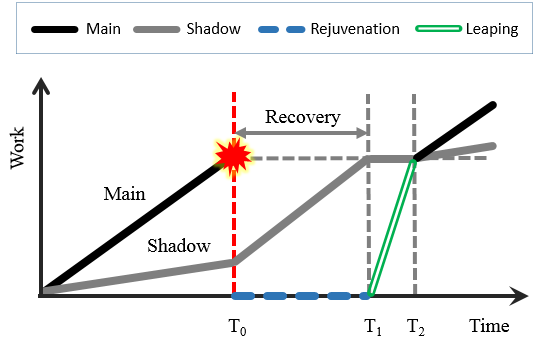
\includegraphics[width=0.6\columnwidth]{Figures/rs_1}
		}
		\subfigure[Non-faulty tasks in different shadowed sets]
		{
			\label{fig:non_faulty_diff}
			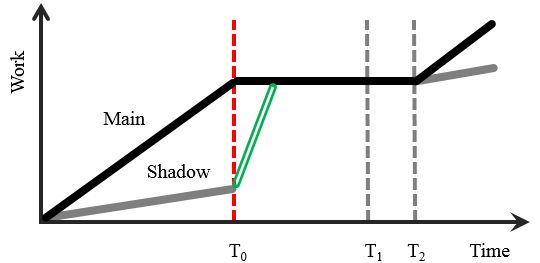
\includegraphics[width=0.6\columnwidth]{Figures/rs_2}
		}
		\subfigure[Non-faulty tasks in the same shadowed set]
		{
			\label{fig:non_faulty_same}
			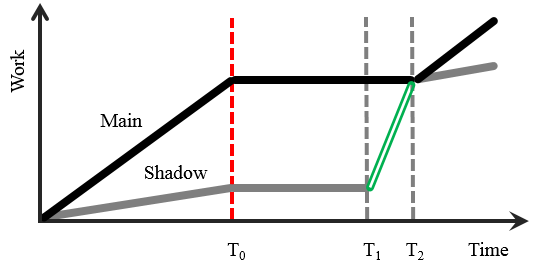
\includegraphics[width=0.6\columnwidth]{Figures/rs_3}
		}
	\end{center}
	%\vskip -0.2in
	\caption{Recovery and rejuvenation after a main process fails.}
	\label{fig:rejuvenation}
\end{figure}
\clearpage
}

Figure~\ref{fig:rejuvenation} and the above description assume that the time for rebooting is no longer than the recovery time. If the new $M_i$ is not yet ready when $S_i$ catches up at $T_1$, however, two design choices are possible. In the first, $S_i$ can assume the role of a main and continue execution. In the second, $S_i$ can wait until the launching of the new $M_i$ is complete. The first option requires that all non-failed processes update their internal mapping to identify the shadow as a new main and continue to correctly receive messages, if any. This not only complicates the implementation, but also requires expensive global coordination that is detrimental to scalability. We, therefore, chose the second design option.

The above analysis focuses on rejuvenating a failed main process. 
Failure of a shadow can be addressed in a similar manner. Each failure requires a rebooting of the target processor to launch replacing process(es), but the only difference is that the leap-provider and leap-recipient are reversed, i.e., the main process becomes the leap-provider and shadow becomes the leap-recipient. Collocation makes the rejuvenation of shadow process slightly more complicated, since a shadow processor failure will impact all the collocated shadows on that processor. Specifically, 
if a shadow processor fails, all the shadows in a shadowed set are lost. To rejuvenate, the failed processor is rebooted and then a new process is launched to replace each of the failed shadow processes. It is to be noted that all the mains can continue execution while rebooting the processor. When the newly launched shadows become ready, rejuvenation-induced leaping is invoked to synchronize every shadow with its main.




\section{Analytical Models}
\vskip -0.2in
In the following we develop analytical models to quantify the expected performance of Leaping Shadows, as well as prove the bound on performance loss due to failures. 
All the analysis below is under the assumption that there are a total of $N$ processors, and $W$ is the application workload.  
$M$ of the $N$ processors are allocated for main processes, each having a workload of $w=\frac{W}{M}$, and the rest $S$ processors are for the collocated shadow processes. %For process replication,
Note that process replication is a special case of Leaping Shadows where $\alpha=1$, so 
$M=S=\frac{N}{2}$ and $w=\frac{2W}{N}$. 

Section~\ref{sec:rejuvenation} discusses rejuvenation to maintain a persistent level of system resilience. In certain situations, the underlying assumption, that failed processor can be rebooted or standby processors are available, may not hold. If this is the case, the scheme discussed in Section~\ref{sec:rejuvenation} becomes invalid, and one has to take the risk that a task may lose both the main and shadow processes, resulting in the entire application being re-executed. To be conservative and emphasize on the benefits of leaping in our assessment of Leaping Shadows, we consider the general case where rejuvenation is not applicable. 

\subsection{Application Fatal Failure Probability}
\label{sec:anal_app_fail}
An application has to roll back when all replicas of a task have been lost. We call this an \textit{application fatal failure}, which is inevitable even when every process is replicated. 
In order to take into account the overhead of rollback in the calculation of completion time and energy consumption, we first 
study the probability of application fatal failure. In this work we assume that once an application fatal failure occurs, execution always rolls back to the very 
beginning. 

The impact of process replication on application fatal failure has been studied in~\cite{casanova_inria_2012} and 
results are presented in terms of Mean Number of Failures To Interrupt (MNFTI), i.e., the mean number of failures to cause an application fatal failure.
Applying the same methodology, we derive the new MNFTI
under collocated Leaping Shadows, 
as shown in Table~\ref{tbl:mnfti}. As each shadowed set can tolerate one failure, the results are 
for different numbers of shadowed sets ($S$). Table~\ref{tbl:mnfti} reveals that the MNFTI almost doubles when the number of shadowed set increases by a factor of 4. At $2^{20}$ shadowed sets, the application is expected to go through 1816 processor failures before observing an interrupt. 
Note that when processes are not shadowed, every failure would interrupt the application, i.e., MNFTI=1. 


\begin{table}[!h]
	\caption{Application Mean Number of Failures To Interrupt (MNFTI) when Leaping Shadows is used. Results are independent of $\alpha=\frac{M}{S}$. }
	\centering
	\small
	\begin{tabular}{|c  |c|c|c|c|c|}
		\hline
		$S$ &  $2^{2}$ &  $2^{4}$ &  $2^{6}$ & $2^8$ & $2^{10}$ \\ 
		\hline
		MNFTI &  4.7 & 8.1 & 15.2 & 29.4 & 57.7 \\
		\hline\hline
		$S$ & $2^{12}$ & $2^{14}$ &  $2^{16}$  & $2^{18}$ & $2^{20}$ \\
		\hline
		MNFTI & 114.4 & 227.9 & 454.7 & 908.5  & 1816.0 \\
		\hline
	\end{tabular}
	\label{tbl:mnfti}
\end{table}

To further quantify the probability of application fatal failure, we use 
$f(t)$ to denote the failure probability density function of each processor, and then $F(t) = \int_0^tf(\tau)d\tau$ is the probability that a processor fails in the next $t$ time. 
Since each shadowed set can tolerate one failure, 
then the probability that a shadowed set with $\alpha$ main processors and 1 shadow processor does not fail by time $t$ is the probability of no failure plus the probability of one failure, i.e., 

\begin{equation}
	P_g = \Big(1-F(t)\Big)^{\alpha+1} + {{\alpha+1} \choose 1}F(t)\times \Big(1-F(t)\Big)^{\alpha}
\end{equation}
and the probability that an fatal failure occurs to an application using $N$ processors within $t$ time is the complement of the probability that
none of the shadowed sets fails, i.e.,

\begin{equation}
	P_a = 1 - ({P_g})^{S}
\end{equation}
where $S=\frac{N}{\alpha+1}$ is the number of shadowed sets.
The application fatal failure probability can then be calculated by using $t$ equal to the expected completion time of the application, which will be modeled in the next subsection.

\subsection{Expected Completion Time}
\label{sec:anal_time}
There are two types of delay due to failures. If a failure does not lead to an application fatal failure, the delay corresponds to the catching up of the shadow of the failing main (see Figure~\ref{fig:jump1}). Otherwise, a possibly larger (rollback) delay will be introduced by an application fatal failure. In the following we consider both delays step by step. 
First we discuss the case of $k$ failures without application fatal failure. Should a failure occur during the recovery of a previous failure, its recovery would overlap with the ongoing recovery. To study the worst case behavior, we assume failures do not overlap, so that the execution is split into $k+1$ intervals, as illustrated in Figure~\ref{fig:progress}. 
$\Delta_i$ ($1\le i \le k+1$) represents the $i^{th}$ execution interval, and $\tau_i$ ($1\le i \le k$) is the recovery time after $\Delta_i$. 


\begin{figure}[!h]
	\begin{center}
		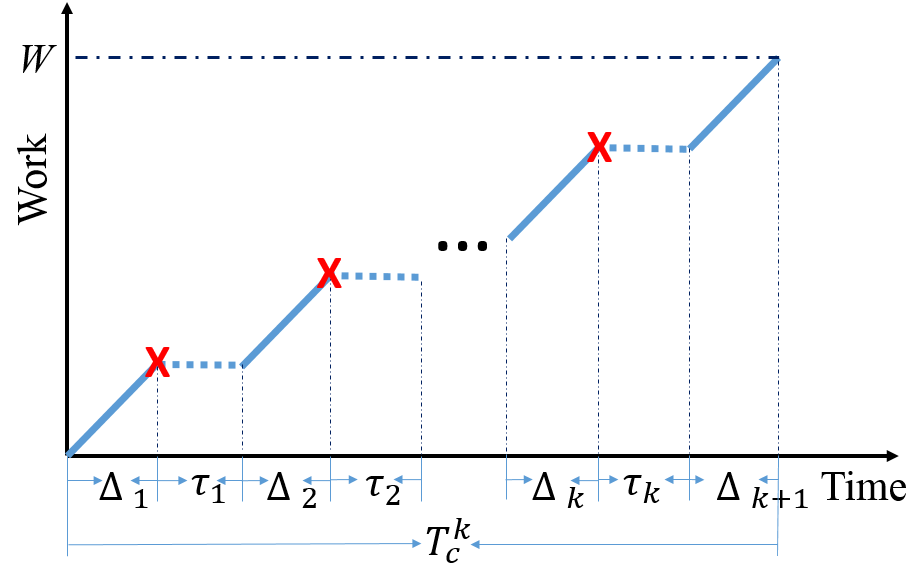
\includegraphics[width=0.8\columnwidth]{Figures/app_progress}
	\end{center}
	\caption{Application progress with shadow catching up delays.}
	\label{fig:progress}
\end{figure}


The following theorem expresses the completion time, $T_c^k$, as a function of $k$.

\begin{theorem}
Assuming that failures do not overlap and no application fatal failure occurs, then using Leaping Shadows, 
	$$T_c^k = w + (1-\sigma_s^b)\sum_{i=1}^k\Delta_i$$
\end{theorem}
\begin{proof}
Leaping Shadows guarantees that all the shadows reach the same execution point as the mains (See Figure~\ref{fig:leap}) after a previous recovery, so every recovery time is proportional to its previous execution interval. 
That is, $\tau_i = \Delta_i \times (1 - \sigma_s^b)$. 
According to Figure~\ref{fig:progress}, the completion time with $k$ failures is 
	$T_c^k = \sum_{i=1}^{k+1}\Delta_i + \sum_{i=1}^k\tau_i = w + (1-\sigma_s^b)\sum_{i=1}^k\Delta_i$
\end{proof}

Although it may seem that the delay would keep growing with the number of failures, 
it turns out to be well bounded, as a benefit of shadow leaping: 

\begin{corollary}
The delay induced by failures is bounded by $(1-\sigma_s^b)w$.
\end{corollary}
\begin{proof}
From above theorem we can see the delay from $k$ failures is $(1-\sigma_s^b)\sum_{i=1}^k\Delta_i$. It is straightforward that, for any non-negative integer of $k$, we have the equation $\sum_{i=1}^{k+1}\Delta_i= w$. As a result, 
$\sum_{i=1}^{k}\Delta_i = w - \Delta_{k+1} \le w$. Therefore, $(1-\sigma_s^b)\sum_{i=1}^k\Delta_i \le (1-\sigma_s^b)w$.
\end{proof}

Typically, the number of failures to be encountered is stochastic. Given a failure distribution, however, we can calculate the probability for a specific value of $k$. We assume that failures do not occur during recovery, so the failure probability of a processor during the execution can be calculated as $P_c = F(w)$. Then the probability that there are $k$ failures among the $N$ processors is 
\begin{equation}
\begin{split}
P_s^{k}= & \dbinom{N}{k}{P_c}^k(1-P_c)^{N-k} \\
\end{split}
\end{equation}

The following theorem expresses the expected completion time, $T_{total}$, considering all possible number of failures. 

\begin{theorem}
Assuming that failures do not overlap, then using Leaping Shadows,
$T_{total} = T_{c} / (1 - P_a)$, where $T_{c} = \sum_{i} T_{c}^{i} \cdot P_s^{i}$.
\end{theorem}
\begin{proof}
Without application fatal failure, the completion time considering all possible values of $k$ can be averaged as $T_{c} = \sum_{i} T_{c}^{i} \cdot P_s^{i}$. If an application fatal failure occurs, however, the application needs to roll back to the beginning. With the probability of rollback calculated as $P_a$ in Section~\ref{sec:anal_app_fail}, the total expected completion time is $T_{total} = T_{c} / (1 - P_a)$.
\end{proof}

Process replication is a special case of Leaping Shadows where the collocation ratio for shadows is 1, so we can apply the above theorem to derive the expected completion time for process replication, when it uses the same amount of processors:

\begin{corollary}
The expected completion time for process replication is $$T_{total} = 2W/N / (1 - P_a)$$.
\end{corollary}
\begin{proof}
Using process replication, half of the available processors are dedicated to shadows so that the workload assigned to each task is significantly increased, i.e., $w=2W/N$. Different from cases where $\alpha \ge 2$, failures do not incur any delay except for application fatal failures. 
As a result, without application fatal failure the completion time under process replication is constant regardless of the number of failures, i.e., $T_c=T_c^k=w=2W/N$. Finally, the expected completion time considering the possibility of rollback is $T_{total} = T_c / (1 - P_a) = 2W/N / (1 - P_a)$.
\end{proof}

\subsection{Expected Energy Consumption}
\label{sec:anal_energy}
Power consumption consists of two parts, dynamic power, $p_d$, which exists only when a processor is executing, and static power, $p_s$, which is constant as long as the machine is on. This can be modeled as $p = p_d + p_s$. Note that in addition to CPU leakage, other components, such as memory and disk, also contribute to static power. 

For process replication, all processors are running all the time until the application is complete. Therefore, the expected energy consumption, $En$, is proportional to the expected execution time $T_{total}$: 
\begin{equation}
En = N \times p \times T_{total}
\label{eq:exp_energy1}
\end{equation} 

Even using the same amount of processors, Leaping Shadows can save power and energy, since main processors are idle during the recovery time after each failure, and the shadows can achieve forward progress through failure-induced leaping. During normal execution, all the processors consume static power as well as dynamic power. During recovery time, however, the main processors are idle and consume only static power, while the shadow processors first perform leaping and then become idle. Altogether, the expected energy consumption for Leaping Shadows can be modeled as 
\begin{equation}
En = N \times p_s \times T_{total} + N \times p_d \times w + S \times p_{l} \times T_l.
\label{eq:exp_energy2}
\end{equation}
with $p_{l}$ denoting the dynamic power consumption of each processor during leaping and $T_l$ the expected total time spent on leaping. 

\begin{theorem}
If no subsequent failure happens before the recovery of the previous failure, then using Leaping Shadows, the upper bound on expected energy consumption is
$(2N * p_s + N * p_d + S * p_{l})*w$.
\end{theorem}
\begin{proof}
From Corollary 1.1 we know that the delay is at most $(1-\sigma_s^b)w \le w$, so $T_{total} \le 2w$. Also, since the leaping time overlaps with the recovery time (delay), $T_l \le (1-\sigma_s^b)w \le w$. Therefore, $En = N * p_s * T_{total} + N * p_d * w + S * p_{l} * T_l \le N * p_s * (2w) + N * p_d * w + S * p_{l} * w = (2N * p_s + N * p_d + S * p_{l})*w$.
\end{proof}










\section{Evaluation}
Careful analysis of the models above leads us to identify several important factors that determine the performance. These factors can be classified into three categories, i.e., system, application, and algorithm. The system category includes static power ratio $\rho$ ($\rho=p_s/p$), total number of processors $N$, and MTBF of each processor; the application category is mainly the total workload, $W$; and collocation ratio $\alpha$ in the algorithm category determines the number of main processors and shadow processors ($N=M+S$ and $\alpha=M/S$). In this section, we evaluate each performance metric of Leaping Shadows,  with the influence of each of the factors considered. %First we calculate the application failure probability for various scenarios. Then we proceed to study the expected energy consumption and completion time under different application failure probabilities. 


\subsection{Comparison to Checkpoint/restart and Process Replication}
\label{eval_comparison}
We compare with both process replication and checkpoint/restart, assuming the same number of processors to use. 
The completion time with checkpoint/restart is calculated with Daly's model~\cite{daly_fgcs_2006} assuming 10 minutes for both checkpointing and restart. The energy consumption is then derived with Equation~\ref{eq:exp_energy1}. It is important to point out that we always assume the same number of processors, so that process replication and Leaping Shadows do not use extra processors for the replicas. 

It is clear from THEOREM 1 that the total recovery delay $\sum_{i=1}^k\tau_i$ is determined by the execution time $\sum_{i=1}^k\Delta_i$, independent of the distribution of failures. 
Therefore, our models are generic with no assumption about failure probability distribution, and the expectation of the total delay from all failures is the same as if failures are uniformly distributed~\cite{daly_fgcs_2006}. Specifically, $\Delta_i = w/(k+1)$, and $T_c^k = w + w*(1-\sigma_s^b)*\frac{k}{k+1}$. Further, we assume that each shadow gets a fair share of its processor's execution rate so that $\sigma_s^b = \frac{1}{\alpha}$. 
To calculate Equation~\ref{eq:exp_energy2}, we assume that the dynamic power during leaping is twice of that during normal execution, i.e., $p_{l}=2*p_d$, and the time for leaping is half of the recovery time, i.e., $T_l=0.5*(T_{total} - w)$. 

The first study uses $N=1$ million processors, effectively simulating future extreme-scale computing environments, and assumes that $W=1$ million hours, and static power ratio $\rho=0.5$. 
Our results show that at extreme-scale, the expected completion time and energy consumption of checkpoint/restart are orders of magnitude larger than those of Leaping Shadows and process replication. Therefore, we choose not to plot a separate graph for checkpoint/restart. 

Figure~\ref{fig:t32} reveals that the most time efficient choice largely depends on MTBF. 
When MTBF is high, Leaping Shadows requires less time as more processors are used for main processes and less workload is assigned to each process. As MTBF decreases, process replication outperforms Leaping Shadows as a result of the increased likelihood of rollback for Leaping Shadows. 
In terms of energy consumption, Leaping Shadows has much more advantage over process replication. For MTBF from 2 to 25 years, Leaping Shadows with $\alpha=5$ can achieve 9.6-17.1\% energy saving, while the saving increases to 13.1- 23.3\% for $\alpha=10$. The only exception is when MTBF is extremely low (1 year), Leaping Shadows with $\alpha=10$ consumes more energy because of extended execution time.

\begin{figure}[!h]
	\begin{center}

		\subfigure[Expected completion time]
		{
			\label{fig:t32}
			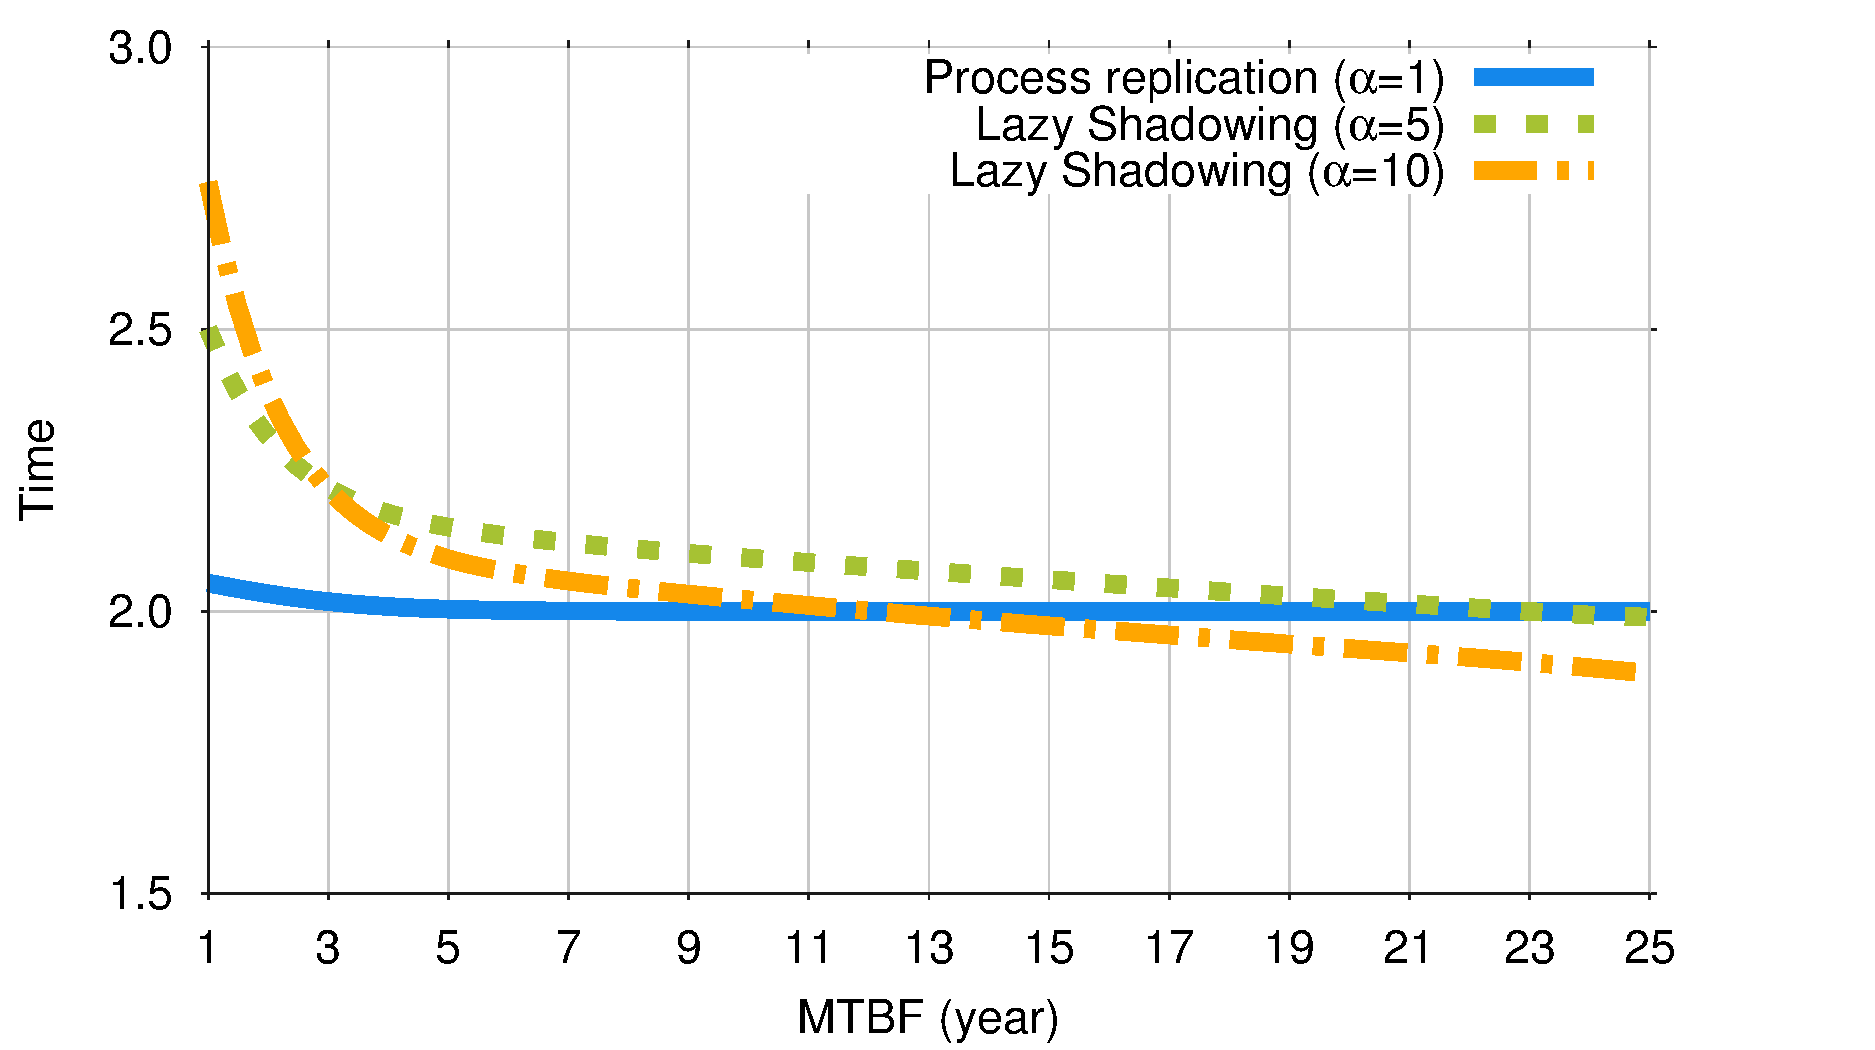
\includegraphics[width=0.7\columnwidth]{Figures/gen_time.pdf}
		} 
		\subfigure[Expected energy consumption]
		{
			\label{fig:e32}
			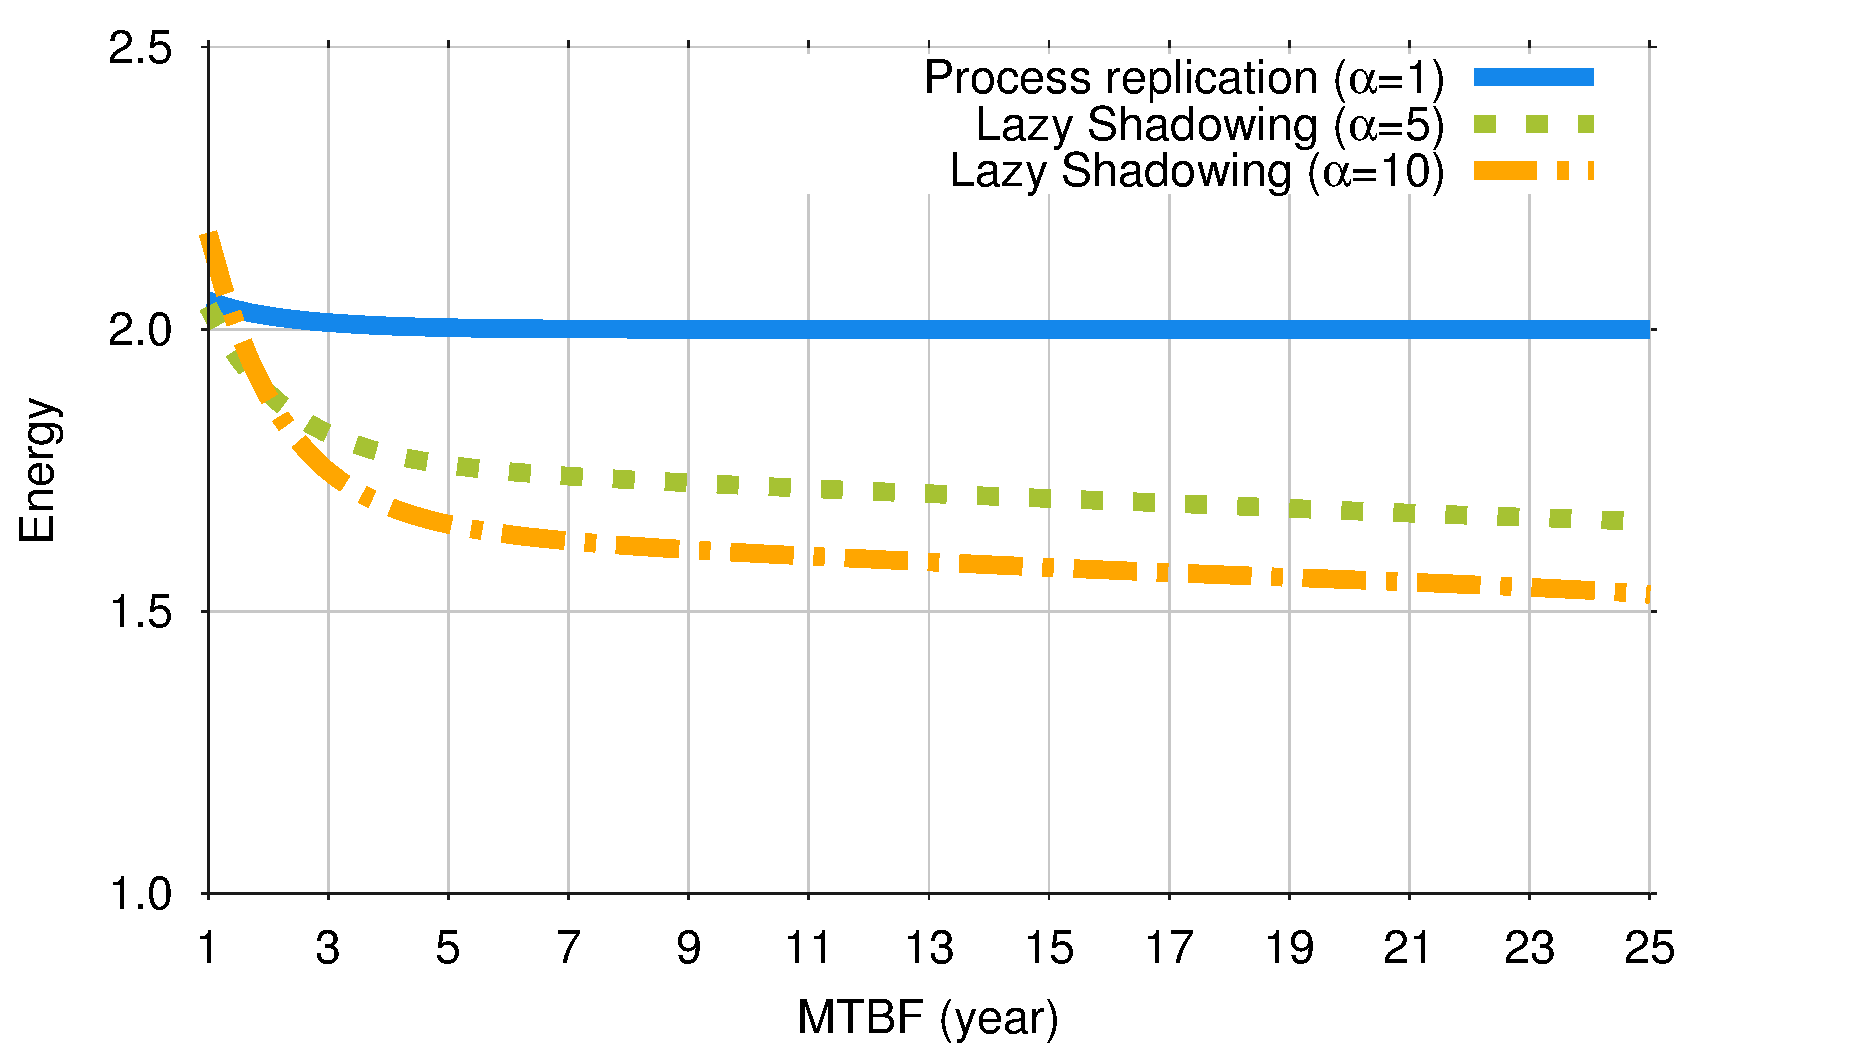
\includegraphics[width=0.7\columnwidth]{Figures/gen_energy.pdf}
		} 
		\caption{Comparison of time and energy for different processor level MTBF. $W=10^6$ hours, $N=10^6$, $\rho=0.5$.}
	\end{center}
	\label{fig:com3}
\end{figure}




\subsection{Impact of Processor Count}
\label{eval_processor}
The system scale, measured in number of processors, has a direct impact on the failure rate seen by the application. To study its impact, we vary $N$ from 10,000 to 1,000,000 with $W$ scaled proportionally, i.e., $W=N$. When MTBF is 5 years, the results are shown in Figure~\ref{fig:n5}. Please note that the time and energy for checkpoint/restart when $N=1,000,000$ are beyond the scope of the figures, so we mark their values on top of their columns. When completion time is considered, Figure~\ref{fig:nt5} clearly shows that each of the three fault tolerance alternatives has its own advantage. Specifically, checkpoint/restart is the best choice for small systems at the scale of 10,000 processors, Leaping Shadows outperforms others for systems with 100,000 processors, while process replication has slight advantage over Leaping Shadows for larger systems. On the other hand, Leaping Shadows wins for all system sizes when energy consumption is the objective. 

When MTBF is changed to 25 years, the performance of checkpoint/restart improves a lot, due to the reduced frequency of checkpointing and decreased need of restarting. However, compelled to rollback every time there is a failure, checkpoint/restart is still orders of magnitude worse in time and energy than that of the other two approaches. Leaping Shadows benefits much more than process replication from the increased MTBF. As a result, Leaping Shadows is able to achieve shorter completion time than process replication when $N$ reaches 1,000,000.

\begin{figure}[!h]
	\begin{center}
		\subfigure[Expected completion time]
		{
			\label{fig:nt5}
			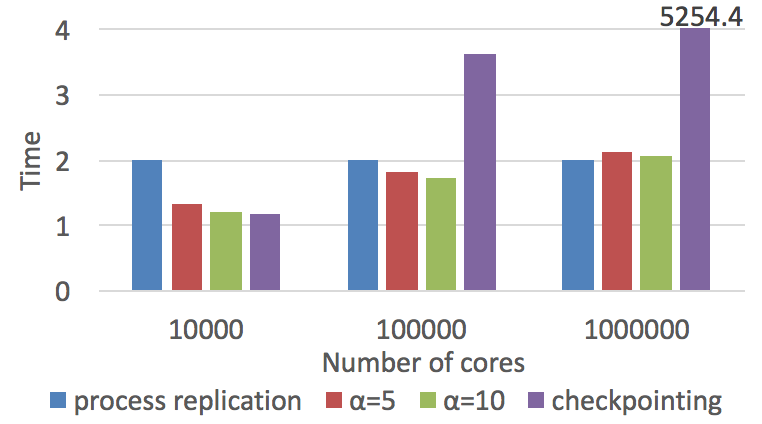
\includegraphics[width=0.7\columnwidth]{Figures/tnt5}
		} 
		\subfigure[Expected energy consumption]
		{
			\label{fig:ne5}
			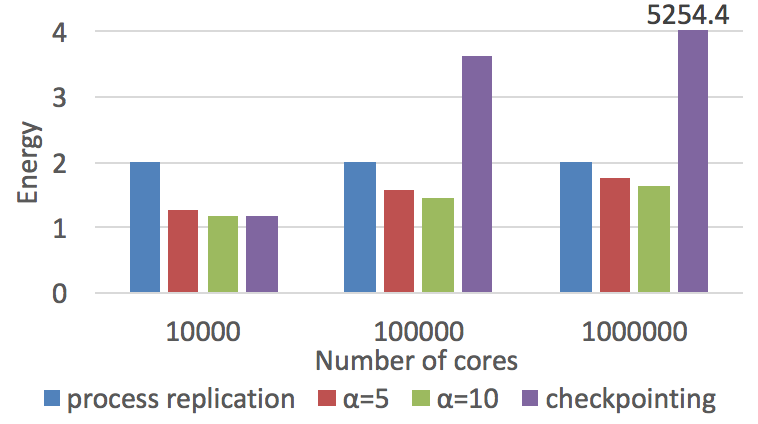
\includegraphics[width=0.7\columnwidth]{Figures/tne5}
		} 
	\end{center}
	\caption{Comparison of time and energy for different number of processors. $W=N$, MTBF=5 years, $\rho=0.5$.}
	\label{fig:n5}
\end{figure}


\subsection{Impact of Workload}
\label{eval_workload}
To a large extent, workload determines the time exposed to failures. With other factors being the same, an application with a larger workload is likely to encounter more failures during its execution. Hence, it is intuitive that workload would impact the performance comparison. 
Fixing $N$ at 1,000,000, we increase $W$ from 1,000,000 hours to 12,000,000 hours. Figure~\ref{fig:w25} assumes a MTBF of 25 years and shows both the time and energy. Checkpoint/restart has the worst performance in all cases. In terms of completion time, process replication is more efficient when workload reaches 6,000,000 hours. Considering energy consumption, however, Leaping Shadows is able to achieve the most savings in all cases. When MTBF of 5 years is used, the difference is that process replication consumes less energy than Leaping Shadows when $W$ reaches 6,000,000.
%\vspace{0.5in}

\begin{figure}[!h]
	\begin{center}
		\subfigure[Expected completion time]
		{
			\label{fig:wt25}
            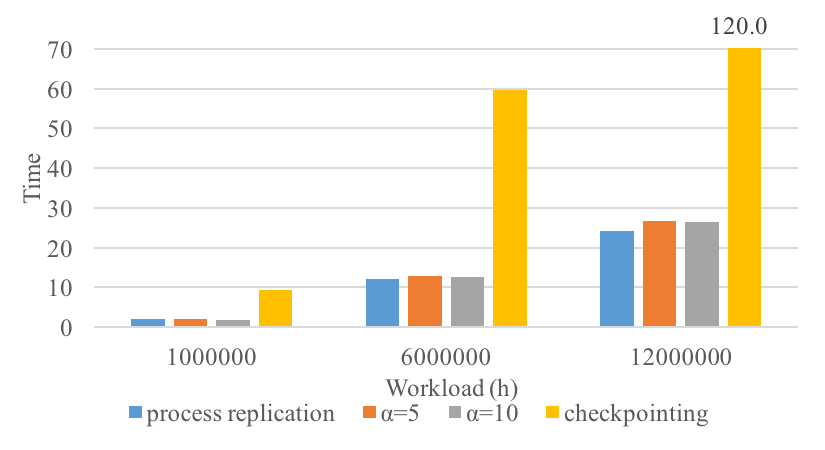
\includegraphics[width=0.7\columnwidth]{Figures/twt25}
			%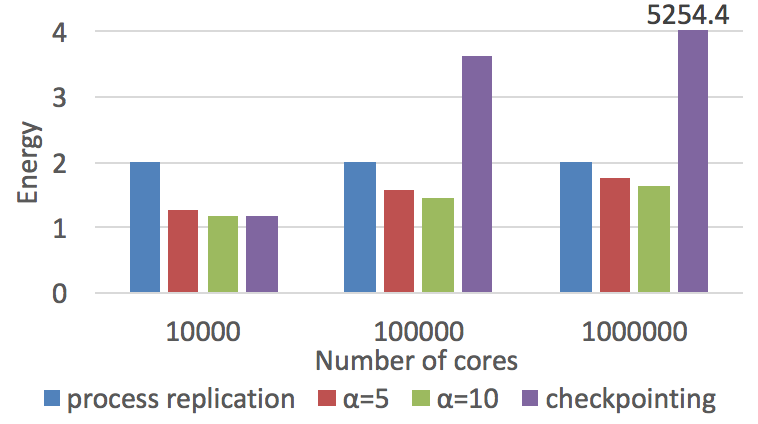
\includegraphics[width=0.7\columnwidth]{Figures/tne5}
		} 
		\subfigure[Expected energy consumption]
		{
			\label{fig:we25}
			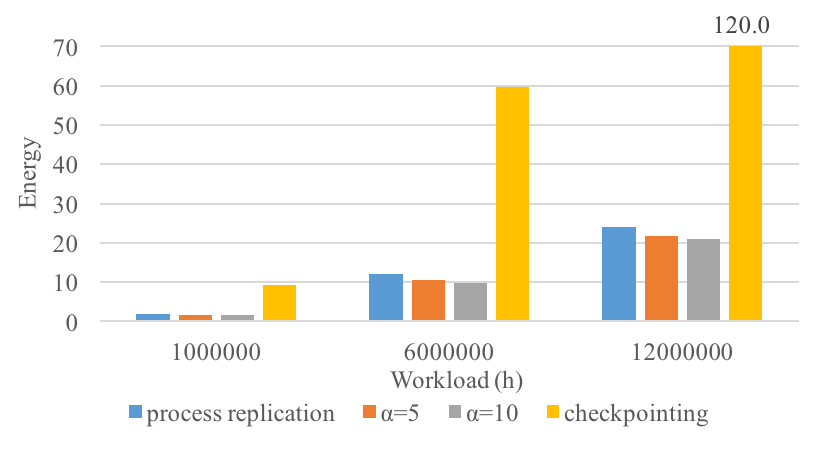
\includegraphics[width=0.7\columnwidth]{Figures/twe25}
            %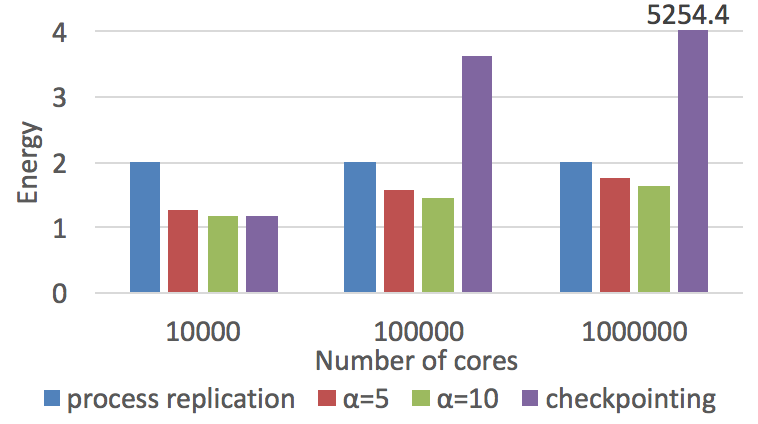
\includegraphics[width=0.7\columnwidth]{Figures/tne5}
		} 
	\end{center}
	\caption{Comparison of time and energy for different workloads. $N=10^6$, MTBF=25 years, $\rho=0.5$.}
	\label{fig:w25}
    \vspace{-0.5in}
\end{figure}

\subsection{Impact of Static Power Ratio}
\label{eval_static_power}
With various architectures and organizations, servers
vary in terms of
power consumption. The static power ratio $\rho$ is used to abstract the
amount of static power consumed versus dynamic power. 
%$\rho$ does not impact the completion time, but power and energy consumption.
Considering modern systems, we vary $\rho$ from 0.3 to 0.7 and study its effect
on the expected energy consumption. The results for Leaping Shadows with $\alpha=5$ are normalized to that of process replication and shown in 
Figure~\ref{fig:power_ratio}. The results for other values of $\alpha$ have similar behavior and thus are not shown. Leaping Shadows achieves
more energy saving when static power ratio is low, since it saves dynamic 
power but not static power. When static power ratio is low ($\rho=0.3$), Leaping Shadows
is able to save 20\%-24\% energy for the MTBF of 5 to 25 years. The saving decreases to 5\%-11\% when $\rho$ reaches 0.7. 

\begin{figure}[!h]
	\begin{center}
		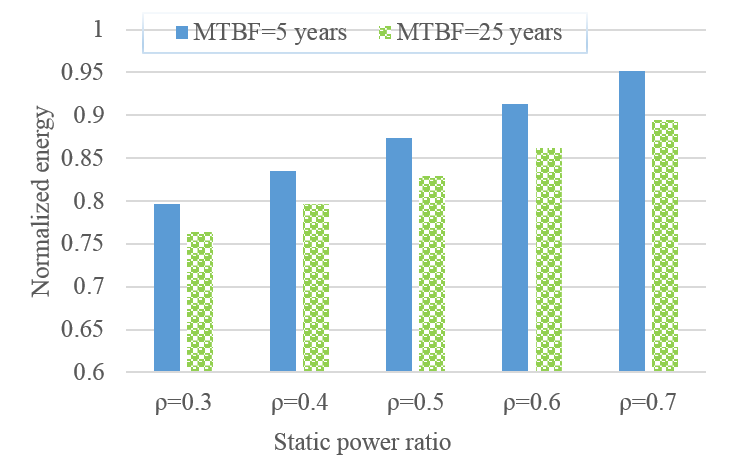
\includegraphics[width=0.7\columnwidth]{Figures/ts_power_5}
	\end{center}
	%\vskip -0.22in 
	\caption{Impact of static power ratio on energy consumption. $W=10^6$ hours, $N=10^6$, $\alpha$=5.}
	\label{fig:power_ratio}
\end{figure}


\subsection{Adding Collocation Overhead}
\label{eval_collocation}
%The last study is conducted to capture the impact on the 
%performance of Leaping Shadows brought by 
%collocation overhead. We re-model the speed of shadows as $\sigma_s^b=\frac{1}{\alpha^{1.5}}$ to simulate the 
%effect of memory thrashing and context switch. 

Leaping Shadows increases memory requirement\footnote{Note that this problem is not intrinsic to Leaping Shadows, as in-memory checkpoint/restart also requires extra memory.} when multiple shadows are collocated. Moreover, this may have an impact on the execution rate of the shadows due to cache contention and context switch. 
To capture this effect,  
we re-model the rate of shadows as $\sigma_s^b=\frac{1}{\alpha^{1.5}}$.
Figure~\ref{fig:comp_vary_fail_speed} shows the impact of collocation overhead on expected energy consumption for Leaping Shadows with $\alpha=5$, with all the values normalized to that of process replication. %The results for other values of $\alpha$ have similar behavior and thus are not shown. 
As expected, energy consumption is penalized because
of slowing down of the shadows. It is surprising, however, that the impact is quite small, with the largest difference being 4.4\%. The reason is that failure-induced leaping can take advantage of the recovery time after each failure and achieve forward progress for shadow processes that fall behind. 
The results for other values of $\alpha$ have similar behavior. 
When $\alpha=10$, the largest difference further decreases to 2.5\%. 

%As expected, both completion time and energy consumption are penalized because
%of slowing down of the shadows. It is surprising, however, that Leaping Shadows with $\alpha=3$ is impacted by the 
%most, while when $\alpha=9$, which means collocating more shadows on each shadow processor, is slightly influenced. After careful analysis,
%we realize that the reason is $\alpha=3$ had the largest values for completion time and energy consumption. Even the percentage of increase after adding the penalty is the smallest, the absolute increase is still the largest. 
%When $\alpha=9$, Leaping Shadows can still achieve 15\%-20\% energy saving with less than 7\% increase in completion time. 

\begin{figure}[!h]
	\begin{center}
		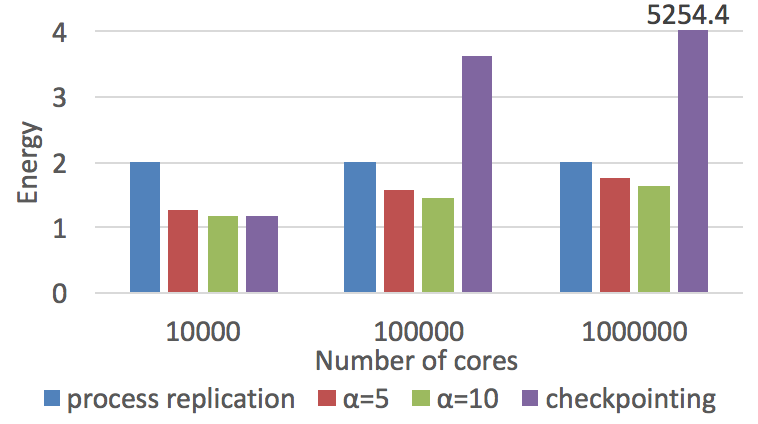
\includegraphics[width=0.7\columnwidth]{Figures/tne5}
        %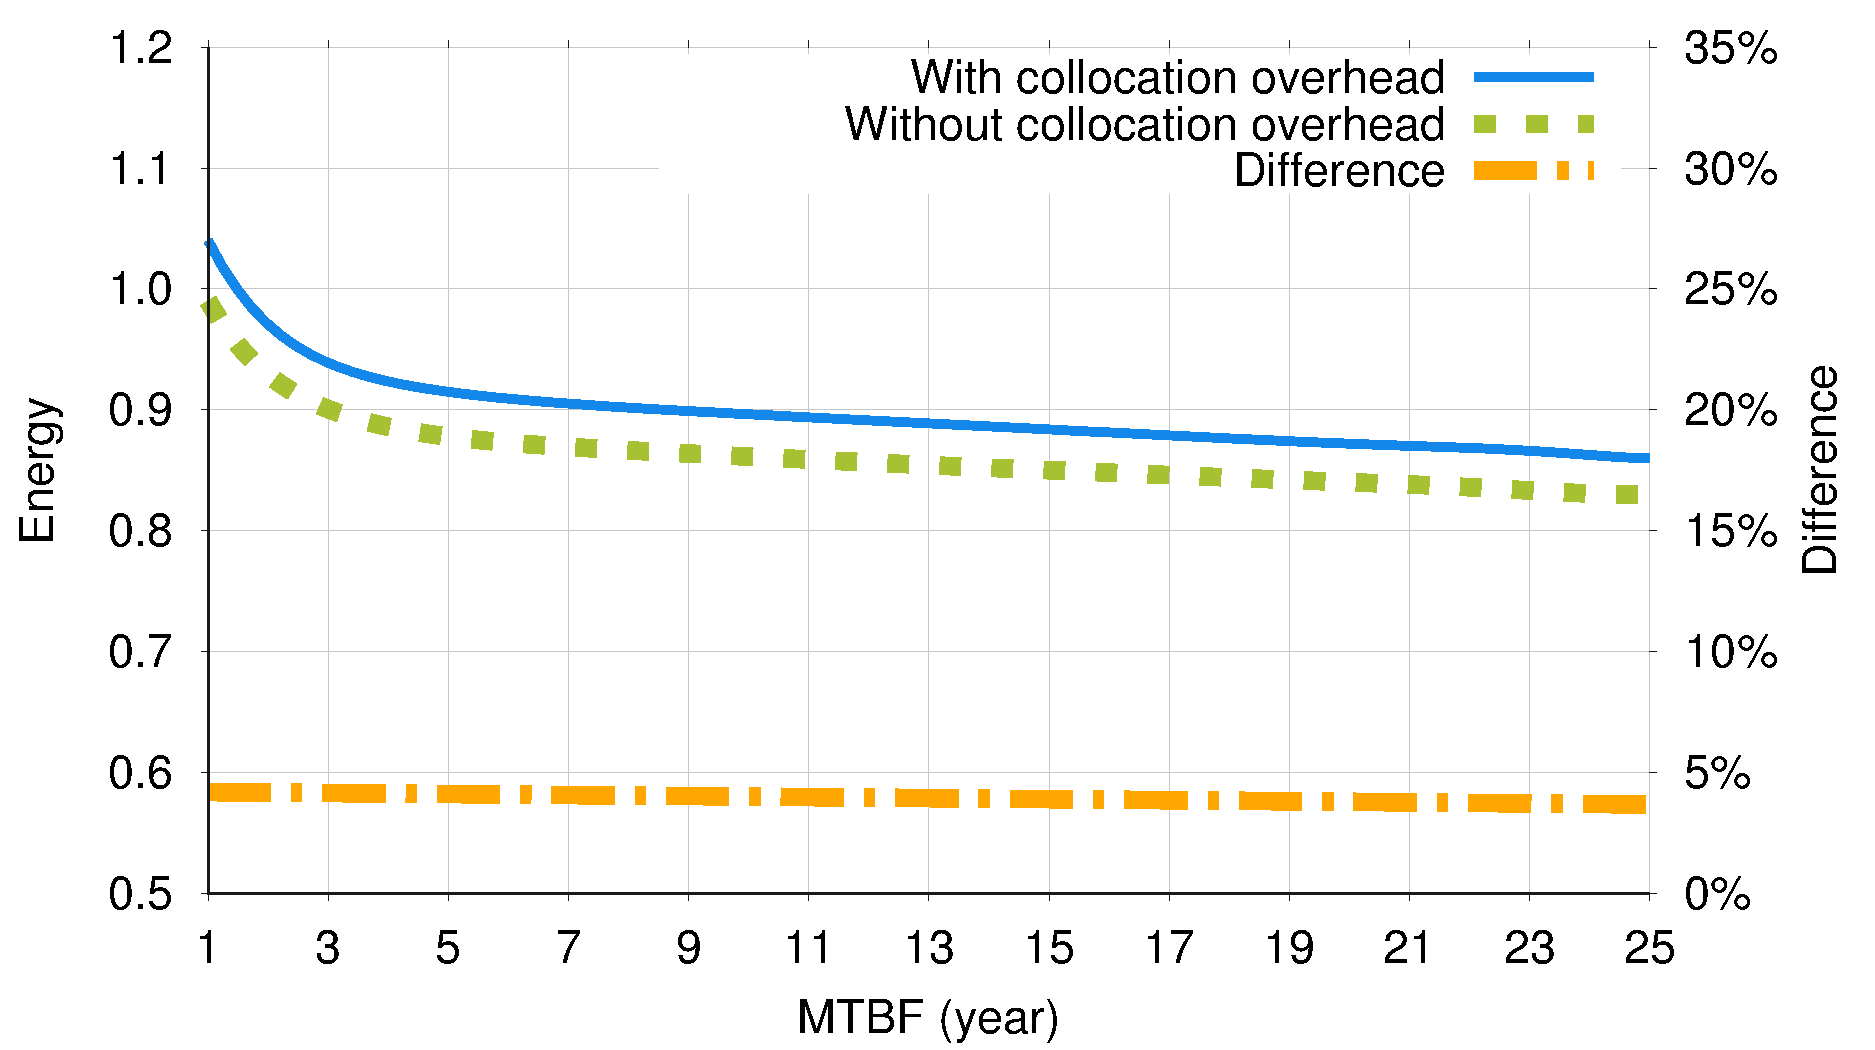
\includegraphics[width=0.7\columnwidth]{Figures/collocation.pdf}
	\end{center}
	\caption{Impact of collocation overhead on energy consumption. $W=10^6$ hours, $N=10^6$, $\rho$=0.5, $\alpha$=5.}
	\label{fig:comp_vary_fail_speed}
\end{figure}






\section{Summary}

As the scale and complexity of HPC systems continue to increase, both the failure rate and power consumption are expected to increase dramatically, making it extremely challenging to deliver the designed performance. Existing fault tolerance methods rely on either time or hardware redundancy. Neither of them appeals to the next generation of supercomputing, as the first approach may incur significant delay while the second one constantly wastes over 50\% of the system resources.

In this work, we present a comprehensive discussion of the techniques that enable Leaping Shadows to achieve scalable resilience in future extreme-scale computing systems. In addition, we develop a series of analytical models to assess its performance in terms of reliability, completion time, and energy consumption. 
Through comparison with traditional process replication and checkpoint/restart, we identify the scenarios where each of the alternatives should be chosen for best performance.










